\documentclass[pdflatex,sn-mathphys-num]{sn-jnl}

\usepackage{graphicx}
\usepackage{multirow}
\usepackage{amsmath,amssymb,amsfonts}
\usepackage{amsthm}
\usepackage{mathrsfs}
\usepackage[title]{appendix}
\usepackage{xcolor}
\usepackage{textcomp}
\usepackage{manyfoot}
\usepackage{booktabs}
\usepackage{float}
\usepackage{subcaption}
\usepackage{tikz}
\usepackage{pgfplots}
\pgfplotsset{compat=1.18}
\usetikzlibrary{arrows.meta, positioning, shapes.geometric}
\usepackage[linesnumbered,ruled,vlined]{algorithm2e}
\usepackage{listings}
\usepackage{stmaryrd}

\theoremstyle{thmstyleone}
\newtheorem{theorem}{Theorem}
\newtheorem{proposition}[theorem]{Proposition}

\theoremstyle{thmstyletwo}
\newtheorem{example}{Example}
\newtheorem{remark}{Remark}

\theoremstyle{thmstylethree}
\newtheorem{definition}{Definition}

\raggedbottom

\begin{document}

\title[Anomaly Detection Using Tensor Decomposition]{Anomaly Detection in Network Traffic Using Tensor Decomposition and IP-Based Multi-Aggregation}

% \author*[1]{\fnm{Jospin Price Yonel} \sur{Mitsouma}}\email{jospinprice@gmail.com}

% \author[2]{\fnm{Pouya} \sur{Ataei}}\email{pouya.ataei.7@gmail.com}

% \author[3,4]{\fnm{Marcellin} \sur{Atemkeng}}\email{m.atemkeng@ru.ac.za}

% \author[1]{\fnm{Emmanuel} \sur{Fouotsa}}\email{emmanuelfouotsa@gmail.com}

% \affil*[1]{\orgdiv{}, \orgname{Center For Cybersecurity and Mathematical Cryptology}, \orgaddress{\street{}, \city{Bamenda}, \postcode{}, \state{}, \country{Cameroon}}}

% \affil[2]{\orgdiv{}, \orgname{Scholarspark.ai}, \orgaddress{\street{68A Hendon Avenue Mount Albert}, \city{Auckland}, \postcode{}, \state{}, \country{New Zealand}}}

% \affil[3]{\orgdiv{Department of Mathematics}, \orgname{Rhodes University}, \orgaddress{\street{PO Box 94}, \city{Grahamstown}, \postcode{6140}, \state{}, \country{South Africa}}}

% \affil[4]{\orgdiv{}, \orgname{National Institute for Theoretical and Computational Sciences}, \orgaddress{\street{}, \city{Stellenbosch}, \postcode{7600}, \state{}, \country{South Africa}}}

\abstract{The proliferation of connected devices in today's interconnected world has created the need for sophisticated anomaly detection systems capable of rapidly identifying abnormal behaviours within massive and heterogeneous data streams. However, traditional anomaly detection systems generally process data in a two-dimensional format, which limits their ability to capture the inherently multidimensional structure of communication data. Tensors provide a principled framework for representing multidimensional data. Nevertheless, tensor-based anomaly detection methods remain predominantly experimental and are subject to inherent limitations that constrain their practical applicability. In this work, we propose a framework that integrates CP decomposition, distinguished by its essential uniqueness (up to permutation and scaling of rank-one components) with IP based multi-aggregation and deep learning, incorporating an automatic rank selection mechanism to optimize the detection of anomalies in network traffic. The method was evaluated using the CIC-IoT 2024 dataset, achieving an accuracy of 99.96\% and a recall of 99.6\%.}

\keywords{Tensor decomposition, Multi-aggregation, Deep Learning, Anomaly detection, Network security}

\maketitle


\section{Introduction}
In today's digitally interconnected landscape, anomaly detection has emerged as an indispensable security mechanism, as our society becomes increasingly reliant on networked infrastructure and digital systems \cite{rcglobal2021} . An anomaly refers to any pattern in data that deviates from expected behaviour \cite{patcha2007overview}. These irregularities often indicate potential security threats such as Denial-of-Service (DoS) attacks, Distributed Denial-of-Service (DDoS) attacks, unauthorised access, or system misconfiguration \cite{eren2023general}. For example, the 2016 Domain name attack exploited the Mirai botnet to generate traffic exceeding $1.2$ Terabits per second, disrupting major websites including Netflix and Twitter \cite{hilton2016dyn}. Similarly, in 2023, Hongkong and Shanghai Banking Corporation's mobile banking services suffered a botnet-driven DDoS attack that targeted API endpoints, resulting in widespread login failures and service disruptions \cite{paloaltonetworks2024}.

This underscores the urgent need for robust anomaly detection systems, especially as the cybersecurity landscape becomes increasingly perilous. According to Cybersecurity Ventures, global damages from cybercrime are projected to reach  \$ $10.5$ trillion annually by 2025, up from \$ $3 $trillion in 2015. These immense losses include business downtime, data breaches, ransom payments, and the high costs associated with recovery and reputational damage. 

Traditional anomaly detection techniques largely rely on classical machine learning algorithms such as Random forest~\cite{biau2016randomforest}, Support Vector Machines (SVM), Principal Component Analysis (PCA)~\cite{marukatat2022tutorial}, Non-negative Matrix Factorization (NMF)~\cite{lee2000nmf}. While effective in certain scenarios, these methods assume a flat, two-dimensional data structure that fails to capture the full complexity of network traffic~\cite{Su2025Robust}. 

Tensors offer a solution to this limitation. As multi-way arrays, tensors generalise the notion of matrices by naturally representing multi-dimensional data. For example, images can be represented as 3D tensors (height, width, channels), videos as 4D tensors (adding the temporal dimension), and network traffic as 4th-order tensors involving source IP, destination IP, time, and features. These higher-order representations preserve the inherent multi-aspect relationships in the data, enabling models to capture more complex patterns and correlations. 

Tensor decomposition is a technique used to extract latent structures from tensors by breaking them down into simpler and interpretable components. Popular decomposition methods include CANDECOMP/PARAFAC (CP) \cite{kolda2009tensor} which is particularly effective for pattern discovery and anomaly detection.
However, there is no straightforward tensor-based optimal method for detecting anomalies in network traffic. Most of the tensor decomposition based models are confronted by the selection of the optimal rank which is a challenging problem, and the complexity of these methods are often high, compromising the flexibility of the methods for real-time applications.


In this paper, we proposed a new method combining Canonical Polyadic (CP) decomposition with multi-aggregation techniques and deep learning models and also integrates an automatic rank selection mechanism to effectively detect anomalies in Internet of Things (IoT) environments. Our approach exploits tensor factorization to capture multi-dimensional relationships in IoT network traffic, while multi-aggregation enables the fusion of diverse features at multiple scales. The deep learning models detect anomalies and the optimal rank can be found. Evaluated on the Canadian Institute of Cybersecurity IoT-2024 datasets, our method demonstrated good performance in detecting combined Denied of Services attacks (DoS) and Distributed Denied of Services attacks (DDoS), outperforming existing traditional models.

 
The key contributions of this work are :
\begin{itemize}
    \item A tensor construction model for the CIC-2024 IoT dataset: We propose a method for constructing tensors from the CIC-2024 IoT dataset based on graph modeling.
    
    \item A new CANDECOMP/PARAFAC based method for detecting anomalies in network traffic : we have combined the CANDECOMP/PARAFAC decomposition with Multi-aggregation method, showing how the complexity of a tensor can be reduced without losing much information and have integrated a deep learning model which detect anomalies and lead the selection of the rank.

\end{itemize}

\section{Related Works}

Tensor decomposition has been widely used in network anomaly detection, work such of \cite{ranjbar2018qanet} proposed an anomaly detection framework that allows users to interactively query a system to identify anomalous entities across heterogeneous information networks. Their approach leverages tensor decomposition and clustering techniques to jointly analyse data from multiple sources such as network, system, and user activity logs. By integrating diverse data modalities, the method successfully reveals complex attack patterns that might remain undetected in isolated log analyses. Additionally, the authors introduced a synthetic network generation model to validate the effectiveness of their approach on both real and synthetic datasets.


The work of \cite{bruns2016ensign} presented the tool ENSIGN which include the implementation of tensor constructions and tensor decomposition algorithms. From it, They to detected anomalous DNS traffic by tracing attack paths over time. Their work provided a practical implementation of tensor methods in operational settings, emphasising the interpretability and scalability of the approach. Despite operational implementation success, ENSIGN suffers from limited scalability to enterprise-level traffic volumes and requires extensive human analyst interaction, reducing automation potential in high-throughput environments.


\cite{xie2018graph} developed Graph-based Tensor Recovery (Graph-TR) method. This model integrates graph Laplacian regularisation with tensor completion to preserve proximity structures during decomposition. The authors highlighted its superior performance in capturing both linear and non-linear correlations in network data, thus improving anomaly detection accuracy. However, their outstanding correlation detection capability is hindered by computational complexity resulting from the huge non-convex problem solved by their algorithm, also by the maintenance and sensitivity to dynamic graph topology changes, limiting effectiveness in rapidly evolving network environments.

In the context of smart grids, \cite{jafarigiv2023tensor} introduced a tensor-based analysis method leveraging data fusion from Information Technology (IT) and Operational Technology (OT) systems. Using both CANDECOMP/PARAFAC (CP) and Higher-Order SVD (HOSVD), they found the low-rank of the tensors generated through co-simulated LTE-based synchrophasor communication scenarios. Their approach effectively isolated anomalies via residual analysis and surpassed the detection performance of Tensor Robust PCA (TRPCA) and NARX neural networks, thus validating the strength of low-rank tensor modelling in cyber-physical systems. However, their approach is limited in smart grid contexts.


\cite{most2023electrical} demonstrated the effectiveness of applying the Canonical Polyadic Alternating Poisson Regression (CP-APR) tensor decomposition within a probabilistic framework to detect anomalies in SCADA systems of the electrical grid.  \cite{zhang2019hybrid} integrated recurrent neural networks with tensor factorization for detecting progressive attacks. Their hybrid approach combines complementary strengths of neural networks' temporal modelling capabilities with tensor methods' interpretability, demonstrating enhanced detection of complex attack sequences that evolve over extended periods.


\cite{sun2006incremental} and \cite{sun2006beyond} pioneered incremental tensor analysis for streaming data and dynamic tensor models for real-time behavioural shift detection. Their work established foundational streaming capabilities for real-time security applications and demonstrated the feasibility of processing continuous network data streams through tensor decomposition methods.


\cite{eren2023general} proposed a method using non-negative CP-based Poisson factorization to detect compromised user credentials, botnets, and spam emails. While the method outperformed state-of-the-art techniques and included an automatic rank selection mechanism, it was complex, highly dependent on factor initialization. 


\cite{streit2021network} worked on an offline and online anomaly detection approach using tensor decomposition to extract the normal subspace from multi-metric time series collected from network routers. Notably, their model operates without requiring packet header inspection, thereby offering privacy-preserving and computationally efficient detection. Their results demonstrated flexibility across different real-world datasets and emphasised the interpretability of the decomposition outcomes. 

\cite{wu2021graph} applied graph neural networks to tensor-based security analysis, demonstrating effective integration of deep learning with tensor methods. Their approach shows promising results in capturing complex network relationships and provides enhanced pattern recognition capabilities through neural network integration. 


Despite evolutionary advances, core limitations persist in the detection of anomalies in dynamic traffic: tensor rank selection, this remains inherently challenging with potentially unstable best low-rank representations \cite{kruskal1977three, kolda2009tensor}, and no universally effective tensor-based anomaly detection method exists. Each approach involves trade-offs between computational complexity, interpretability, and generalization across diverse environments. 


In this work, we exploited these work to construct a new framework which integrate the CP decomposition, deep learning,  multi-aggregation and the rank selection strategy to optimize the detection capability of anomalies.


The remainder of this paper is structured as follows: Section 3 presents the methodology, providing a detailed explanation of our proposed framework; Section 3 describes the experimental evaluation conducted on the CIC-2024 IoT dataset; and Section 4 concludes with a summary of findings and future research directions.
  

\section{Data and Methodology}
The proposed methodology consists of successive stages, beginning with preprocessing of the CIC-IoT 2024 dataset, followed by its tensorization.. The resulting tensor is subsequently decomposed to extract its underlying structure, after which an arbitrary tensor derived from an identical tensorization process is projected onto the obtained latent space. The residuals generated from this projection are systematically aggregated and employed as input features for deep learning models, which are trained across different tensor rank. Finally, comprehensive model evaluation is conducted and the optimal rank is determined based on established performance metrics. Figure ~\ref{fig:framework}  provides an overall representation of this methodological framework.
\begin{figure}
    \centering   \includegraphics[width=1.18\linewidth]{Framework_Overview.png}
    \caption{Overview of the proposed framework : This figure outlines the }
    \label{fig:framework}
\end{figure}

\subsection{Dataset}
The dataset used in our study is the Canadian Institute for Cybersecurity IoT 2024 Dataset for Anomaly Detection \cite{rabbani2024iot-diad} which contains network traffic flows of 105 IoT devices communications.The malicious traffic are categorized into several types of attacks, such as DDoS, DoS, Spoofing, and Brute Force. In the author website, that dataset is split into several repositories, each containing a specific kind of traffic. Our experimental analysis began with the selection of seven datasets from the CIC IoT 2024 repository. Among these, four correspond to benign traffic, one captures DDoS HTTP attack traffic, and the remaining two represent DoS HTTP attack traffic. After cleaning the datasets, we obtained the following dimensions, respectively:
$(183,630 \times 85)$, $(84,526 \times 85)$, $(91,279 \times 85)$, $(38,895 \times 85)$, $(505,720 \times 85)$, $(932,513 \times 85)$, and $(710,231 \times 85)$.

The raw traffic data consist of flows containing various numerical and categorical features. The preprocessing phase involved firstly removing undesirable entries, including missing, infinite, and NaN values, and adding labels for anomalous and benign traffic.

In the selected datasets, significant temporal heterogeneity was observed, with data collection periods extending up to two months across the different datasets. To mitigate this variability, a relative time variable was introduced, defined as follows:

\begin{equation}
t_{\text{rel}}^{(i)} = t_{\text{abs}}^{(i)} - t_{\min}^{(i)},
\end{equation}
\noindent where $t_{\text{abs}}^{(i)}$ denotes the absolute timestamp, $t_{\min}^{(i)} = \min\{t : t \in \mathcal{T}_i\}$ represents the minimum timestamp in dataset $i$, and $\mathcal{T}_i$ is the set of all timestamps within dataset $i$. 

The relative time variable computed synchronised the datasets. This step was essential, as the temporal heterogeneity observed in the CIC IoT 2024 dataset reflects a common real-world challenge in network security research. Our relative time construction effectively mitigates this issue by providing a unified temporal reference frame, thereby enabling consistent cross-dataset analyses.

The preprocessing is followed by Aggregating traffic into fixed-duration time windows of five minutes. Since in this study, we focused on the detection of two combined attacks ( DoS and DDoS ), four relevant numerical attributes were selected including flow byte rate, flow packet rate, flow duration, and counts. 

Finally, the selected features are normalized using standard scaling techniques to ensure consistent value ranges, which improved convergence during tensor decomposition and model training.

As  final step in our data preprocessing, we constructed three datasets containing one hour of traffic each. The Normal Dataset, consisting of purely benign network traffic and serves as a reference for normal behaviour, the Training Dataset, containing both benign and malicious samples intended for training the models, and the Testing Dataset, containing the same mixture of benign and malicious traffic as the Training Dataset and is used to evaluate model performance, each with shape  $(21587, 88)$,$(409623, 88)$,$
(84709, 88)$ respectively. 





\subsection{Tensor Construction}
The construction of the CIC-IoT 2024 dataset tensor was done using the time-binned graph tensor strategy. This approach generates a dynamic graph where the nodes represent the IP addresses and the edges are vectors capturing the communication features exchanged between them. 

Formally, for each time window $t$, we define the graph $G_t = (V, E_t)$ where $V$ represents the set of all observed IP addresses and $E_t \subseteq V \times V$ denotes the set of directed edges at time $t$. We considered four key flow characteristics; flow byte rate, flow packet rate, duration, and packet counts. The dynamic nature of this graph emerges from the time-varying edge set, reflecting the evolving communication patterns in the network. 

This construction yields a 4D tensor $\mathcal{X} \in \mathbb{R}^{I_1 \times I_2 \times I_3 \times 4}$, where the tensor modes correspond to time windows (cardinality $I_1$), source IP addresses (cardinality $I_2$), destination IP addresses (cardinality $I_3$), and four numerical features. The resulting tensor $\mathcal{X}$ effectively captures the temporal evolution of multivariate communication patterns across all source-destination pairs, providing a comprehensive representation of network behaviour  over time. Figure ~\ref{fig:tensor_3d} illustrates the tensor obtained at time window $t$.

\begin{figure}[H]
    \centering
    \includegraphics[width=0.8\linewidth]{Sh (1).png}
    \caption{CIC Tensor at Time Window $t$: This figure shows the CIC IoT 2024 tensor at a given time window. Black points represent benign traffic, while orange points indicate malicious traffic. The tensor is structured in three dimensions: source, destination, and feature.}

    \label{fig:tensor_3d}
\end{figure}

\subsection{CP Tensor Decomposition}
Here we discuss the CP decomposition and its computation. 
Let consider $\mathcal{X} \in \mathbb{R}^{I_1 \times I_2 \times I_3 \times I_4}$ a $4$-th order tensor. The CANDECOMP/PARAFAC (CP) decomposition consists of representing $\mathcal{X}$ as a sum of $R$ rank-one tensors:

\begin{equation}
\mathcal{X} \approx \sum_{r=1}^{R} \mathbf{a}_r^{(1)} \circ \mathbf{a}_r^{(2)} \circ \mathbf{a}_r^{(3)} \circ \mathbf{a}_r^{(4)},
\label{eq:cp-basic}
\end{equation}

\noindent where $\mathbf{a}_r^{(n)} \in \mathbb{R}^{I_n}$ denotes the $r$-th factor vector in mode $n$ and $\circ$ denotes the outer product. When weights are incorporated, the decomposition becomes:
\begin{equation}
\mathcal{X} \approx \sum_{r=1}^{R} \lambda_{r} \, \mathbf{a}_r^{(1)} \circ \mathbf{a}_r^{(2)} \circ \cdots \circ \mathbf{a}_r^{(N)},
\label{eq:cp-lambda}
\end{equation}

\noindent where $\lambda_r$ represents the weight of the $r$-th component. This decomposition can be expressed using factor matrices as: 
\begin{equation}
\mathcal{X} \approx \llbracket {\lambda}; \mathbf{A}^{(1)}, \mathbf{A}^{(2)}, \ldots, \mathbf{A}^{(N)} \rrbracket,
\label{eq:kruskal-form}
\end{equation}
\noindent where
\(
\mathbf{A}^{(n)} = \llbracket\mathbf{a}_{1}^{(n)}, \mathbf{a}_{2}^{(n)}, \cdots, \mathbf{a}_{R}^{(n)} \rrbracket \in \mathbb{R}^{I_n \times R}, 
\)
$\lambda \in \mathbb{R}^{R}$, and $\llbracket \cdot \rrbracket$ denotes the Kruskal operator \cite{kruskal1977three}. Note that, 
the the mode-$n$ unfolding of $\mathcal{X}$ satisfies the relation
\begin{equation} \label{eq:mode_n_unfolding}
\mathbf{X}_{(n)} \approx \mathbf{A}^{(n)} \, \boldsymbol{\Lambda} 
\left( \mathbf{A}^{(4)} \odot \cdots \odot \mathbf{A}^{(n+1)} \odot \mathbf{A}^{(n-1)} \odot \cdots \odot \mathbf{A}^{(1)} \right)^\top,
\end{equation}
where $\boldsymbol{\Lambda} = \operatorname{diag}(\lambda_1, \dots, \lambda_R)$ contains the pattern weights, and $\odot$ denotes the Khatri-Rao product \cite{kruskal1977three}.


A key advantage of CP decomposition lies in its essential uniqueness, which holds up to permutation and scaling of the rank-one components. This uniqueness property is particularly important as it mitigates the orthogonality limitations typically associated with matrix decompositions. A classical result by Kruskal provides a sufficient condition under which this uniqueness is guaranteed:
\begin{equation}
k_{\mathbf{A}^{(1)}} + k_{\mathbf{A}^{(2)}} + \cdots + k_{\mathbf{A}^{(N)}} \geq 2R + (N-1),
\end{equation}

\noindent where $k_{\mathbf{A}^{(n)}}$ is the Kruskal rank defined as the maximum number of linearly independent columns of matrix $\mathbf{A}^{(n)}$. This condition ensures that patterns extracted through CP decomposition are identifiable and reproducible.



To compute the CP decomposition of a tensor, several algorithms are used. For our problem, we employed the Alternating Least Squares (ALS) algorithm, which is particularly well-suited for large-scale datasets. While the CP problem seeks to find $R$ rank-one tensors, 
the Alternating Least Squares (ALS) algorithm solves the problem by updating one factor matrix at a time while keeping others fixed. At each iteration and for a given mode $n$, we solve:

\begin{equation}
\min_{\mathbf{A}^{(n)}} \left\| \mathcal{X}_{(n)} - \mathbf{A}^{(n)} \, \boldsymbol{\Lambda} 
\left( \mathbf{A}^{(4)} \odot \cdots \odot \mathbf{A}^{(n+1)} \odot \mathbf{A}^{(n-1)} \odot \cdots \odot \mathbf{A}^{(1)} \right)^\top 
\right\|_F^2,
\end{equation}
\noindent where $\left|\cdot\right|_{F}$ denotes the Frobenius norm and $\top$ represents the transpose operator. This is a convex optimization problem with respect to the factor matrix $\mathbf{A}^{(n)}$, which ensures the existence of a unique global minimum when the other factor matrices are fixed. The optimal solution is
\begin{equation}
\mathbf{A}^{(n)} = \mathcal{X}_{(n)} 
\left( \bigodot_{i \neq n} \mathbf{A}^{(i)} \right) 
\mathbf{G}^{-1},
\end{equation}

\noindent where 
$
\mathbf{G} = \ast_{i \neq n} \left( \mathbf{A}^{(i)\top} \mathbf{A}^{(i)} \right) 
$ and $\ast$ denotes the Hadamard product (element-wise). 

The process of computing the CP decomposition with the ALS algorithm begins by initializing all factor matrices $\mathbf{A}^{(i)}$, then iteratively updating each factor using the optimal solution given in equation (8) and repeat until convergence. The following is the entire algorithm taken in the paper of \cite{kruskal1977three}

\begin{algorithm}[H]
\caption{CP Decomposition using ALS }
\KwIn{Tensor $\mathcal{X}$, target rank $R$, max iterations $T$, tolerance $\epsilon$}
\KwOut{Factor matrices $\mathbf{A}^{(1)}, \ldots, \mathbf{A}^{(N)}$ and fit score}

Initialize $\mathbf{A}^{(1)}, \ldots, \mathbf{A}^{(N)}$ randomly or using prior knowledge\;
$\text{fit}_{\text{old}} \gets 0$\;

\For{$\text{iteration} \gets 1$ \KwTo $T$}{
    \For{$n \gets 1$ \KwTo $N$}{
        $\mathbf{V} \gets \bigodot_{i \neq n} \mathbf{A}^{(i)}$\; 
        $\mathbf{G} \gets \prod_{i \neq n} \left( \mathbf{A}^{(i)\top} \mathbf{A}^{(i)} \right)$\; 
        $\mathbf{A}^{(n)} \gets \mathcal{X}_{(n)} \mathbf{V} \mathbf{G}^{-1}$\;
        Normalize columns of $\mathbf{A}^{(n)}$\;
    }
    Compute fit: $\text{fit} \gets 1 - \frac{\|\mathcal{X} - \hat{\mathcal{X}}\|_F}{\|\mathcal{X}\|_F}$\;
    \If{$|\text{fit} - \text{fit}_{\text{old}}| < \epsilon$}{
        \textbf{break}\;
    }
    $\text{fit}_{\text{old}} \gets \text{fit}$\;
}
\Return $\mathbf{A}^{(1)}, \ldots, \mathbf{A}^{(N)}, \text{fit}$\;
\end{algorithm}



\subsection{Normal space Projection}
Consider the tensor \(\mathcal{X} \in \mathbb{R}^{I_1 \times I_2 \times I_3 \times I_4}\) having a CP decomposition as previously defined. At each time step \(i \in \{1, \dots, I_1\}\), we can write the time slice of \(\mathcal{X}\) as:

\begin{equation}
\mathcal{X}_{i,:,:,:} \approx \sum_{r=1}^{R} \mathbf{a}_{ri}^{(1)} \cdot \left( \mathbf{a}_r^{(2)} \circ \mathbf{a}_r^{(3)} \circ \mathbf{a}_r^{(4)} \right).
\end{equation}

\noindent We observe that at each time step \(i\), there exists a vector \(\mathbf{a}_{ri}^{(1)}\) such that the above approximation holds. Given a new tensor \(\mathcal{Y} \in \mathbb{R}^{I_1 \times I_2 \times I_3 \times I_4}\), we assume it to follow the same structural as \(\mathcal{X}\)  . This implies that each time slice \(\mathcal{Y}_{i,:,:,:}\) can be naturally projected onto the subspace spanned by \(\left\{\mathbf{a}_r^{(2)} \circ \mathbf{a}_r^{(3)} \circ \mathbf{a}_r^{(4)}  \right\}_{r=1}^{R}
\). Specifically, we seek a vector \(\hat{\mathbf{a}}_{i}^{(1)} \in \mathbb{R}^{1 \times R}\) such that:
\begin{equation}
\mathcal{Y}_{i,:,:,:} \;\approx\; 
\sum_{r=1}^{R} \hat{a}^{(1)}_{ri} \cdot 
\left( \mathbf{a}_r^{(2)} \circ \mathbf{a}_r^{(3)} \circ \mathbf{a}_r^{(4)} \right)
\qquad \forall i \in I_1.
\end{equation}



\noindent This problem can be reformulated as a least-squares optimization task:
\begin{equation}
\min_{\hat{\mathbf{a}}_{i}^{(1)}} \left\| \mathcal{Y}_{i,:,:,:} - \sum_{r=1}^{R} \hat{\mathbf{a}}_{ri}^{(1)} \cdot \left( \mathbf{a}_r^{(2)} \circ \mathbf{a}_r^{(3)} \circ \mathbf{a}_r^{(4)} \right)\right\|_F^2,
\end{equation} and the optimal solution is given by: 

\begin{equation}
\hat{\mathbf{a}}_{i}^{{(1)}\top} = \left(\mathbf{Z}^\top \mathbf{Z} \right)^{-1} \mathbf{Z}^\top vec(\mathcal{Y}_{i,:,:,:}),
\end{equation}
where \(\mathbf{Z}=\left( \mathbf{a}_r^{(2)} \circ \mathbf{a}_r^{(3)} \circ \mathbf{a}_r^{(4)} \right)_{1\leq r\leq R} \in \mathbb{R}^{I_2I_3I_4 \times R}\).
Note \(\mathbf{\hat{A}}^{(1)} \in \mathbb{R}^{I_1 \times R}\)  the matrix of learned temporal coefficients, where each  \(\hat{\mathbf{a}}_i\) corresponds to the $i$-th row. We can then reconstruct the projected tensor \(\mathcal{\hat{Y}}\), which lies in the learned subspace \(
\mathcal{\hat{Y}} \approx [\![\mathbf{\hat{A}}^{(1)}, \mathbf{A}^{(2)}, \mathbf{A}^{(3)}, \mathbf{A}^{(4)}]\!]
\) and deduce the global residual tensor $\mathcal{R}$ as:
\(\mathcal{R} = \mathcal{Y} - \mathcal{\hat{Y}}.\)
These residuals are used to measure the deviation of the observed data from the learned normal subspace and can easily allow us to characterize normal from abnormal behaviours.

\subsection{Enhanced multi-perspective aggregation}

To enhance the detection capacity, we adopted an aggregation strategy at the IP address level on the residual tensors. This strategy consists of aggregating the residuals using first the source IP addresses and second the destination IP addresses in order to obtain a 360-degree view of the resulting scores. In our study, we focus on the source IP-based aggregation approach. Let us consider the residual tensor \(\mathcal{R}\) obtained from projection, we compute a new 3 order score tensor \(\mathcal{S} \in \mathbb{R}^{I_1 \times I_3 \times I_4}\), defined as:
\begin{equation}
    \mathcal{S}_{i, j, k} = \sum_{s=1}^{I_2} |\mathcal{R}_{i, s, j, k}|.
\end{equation}
\noindent This aggregation allowed us to focus on the behaviour of destination IPs over time and served as the basis for subsequent anomaly detection. Optionally, we could reduce further by computing a global anomaly score per Dst IP and time using the \(L_2\) norm over features:
\[
\mathcal{G}_{i,k} = \left( \sum_{j=1}^{I_3} \left( \sum_{s=1}^{I_2} |\mathcal{R}_{i, s, j, k}| \right)^2 \right)^{1/2}.
\]
\noindent From these scores, we formed a dataset of 6 or 7 features depending on if label exists or not and we used it as input of a deep learning model.

A fundamental challenge in tensor decomposition-based frameworks is the selection of an appropriate rank \(R\). An insufficiently small rank may result in underfitting and the omission of essential structural patterns, whereas a large rank introduces the risk of overfitting and unwarranted complexity. To address the issue of suboptimal rank selection, we adopted a model selection methodology that determines the optimal rank by minimizing a task-specific loss function \( \mathcal{L}(\phi_{R_n}) \), such as:
\[
    \mathcal{L}(\phi_{R_n}) = 
    \begin{cases}
        \mathbb{E}_{(\mathbf{s}, y) \sim \mathcal{D}_{\text{val}}} \left[ \ell_{\text{CE}}\left(\phi_{R_n}(\mathbf{s}), y \right) \right] & \text{(supervised)} \\
        \mathbb{E}_{\mathbf{s} \sim \mathcal{D}_{\text{val}}} \left[ \|\mathbf{s} - \phi_{R_n}(\mathbf{s})\|^2 \right] & \text{(unsupervised)},
    \end{cases}
\]
and the optimal rank is given by: 
\(
    \hat{R} = \arg\min_{R_n \in \mathcal{R}} \mathcal{L}(\phi_{R_n}). 
\)  Here, \(\phi_{R_n}\) 
denotes the deep learning model trained with rank \(R_n\)
and the optimal rank is selected as the one for which the model achieves the best balance in performance evaluation.   

\subsection{Deep learning classifiers and evaluations}
Scores obtained from the enhanced multi-perspective step were utilized to construct a dataset comprising 6 or 7 features depending on whether labels were available or not. The dense deep learning model having architecture shown in figure~\ref{Deeplearning} was trained.
\begin{figure}[H]
    \centering
\includegraphics[width=0.35\linewidth]{neuro network.png}
    \caption{Deep learning architecture used our the experimentation. It exhibits the order Activation (ReLU) $\rightarrow$ Batch Normalization (BN) $\rightarrow$ Dropout }
    \label{Deeplearning}
\end{figure}
The configuration Activation (ReLU) $\rightarrow$ Batch Normalization (BN) $\rightarrow$ Dropout was adopted based on the findings of \cite{ding2019acnet}, who demonstrated that normalizing post-activation values can better stabilizes gradient flow and reduces internal covariate shift more effectively than the traditional BN $\rightarrow$ ReLU ordering. This observation was confirmed in our experiments, where the BN $\rightarrow$ ReLU arrangement exhibited instability during training with our dataset. By applying BN after ReLU, the network normalizes sparse, non-negative activations, thereby mitigating dead neurons and improving training dynamics \cite{tensorflow_addons2021}. Dropout is then applied to the normalized activations to directly regularize them, suppress extreme values, and enhance generalization \cite{li2019understanding}.

Furthermore, the progressive reduction in layer width (60 $\rightarrow$ 40 $\rightarrow$ 20) alongside decreasing dropout rates (0.3 $\rightarrow$ 0.1) is guided by the information bottleneck principle. In this framework, stronger regularization in early layers helps prevent overfitting, while later layers preserve discriminative features \cite{labach2019survey, rippel2015spectral}. Overall, this design achieves a balance between stability and performance, building upon modern insights beyond the original Batch Normalization formulation \cite{ioffe2015batch}.

To evaluate our model, we used standard classification metrics, including accuracy, precision, recall, and the F1-score, defined as follows:
\begin{align}
\text{Accuracy} &= \frac{TP + TN}{TP + TN + FP + FN}\\
\text{Precision} &= \frac{TP}{TP + FP}\\
\text{Recall} &= \frac{TP}{TP + FN}\\
\text{F1} &= 2 \times \frac{\text{Precision} \times \text{Recall}}{\text{Precision} + \text{Recall}}
\end{align}
where :
 TP is the number of true predicted attacks,
TN  is the number of true non attacks,
FP is the number of non attacks predicted as attacks, and 
FN is the number of attacks predicted as normal.






\section{Results}
In this section, we present our findings and their interpretations.   After completing all preprocessing steps, we proceeded to the tensor construction process, as described in the previous section. In this phase, three tensors were constructed; $\mathcal{X}_{\text{normal}}$, $\mathcal{X}_{\text{train}}$, and $\mathcal{X}_{\text{test}}$, each with shape $(13, 822, 1313, 4)$, corresponding to the three previously created datasets and each tensor contained 56,122,872 elements, with sparsity levels of $1.8 \times 10^{-4}\%$, $4.8 \times 10^{-4}\%$, and $3.77 \times 10^{-4}\%$ respectively. 

This sparsity reflects the realistic nature of network traffic, particularly in IoT environments where communication typically occurs between a limited number of devices rather than across fully connected networks. Furthermore, since the dataset covered only one hour of network activity, many potential connections between devices had not yet been established, further contributing to the sparsity observed. 
\begin{figure}
    \centering
    \includegraphics[width=.8\textwidth]{Compression Graph.png}
    \caption{Compression Graph showing reconstruction error vs. rank. It shows the improvement quality of the decomposition}
    \label{fig:Compression graph}
\end{figure}
\subsection{Network Traffic Behaviour Extraction}
Normal tensor $\mathcal{X}_{\text{normal}}$ was decomposed using $16$ different rank values, yielding four factor matrices for each decomposition : $\mathbf{A} \in \mathbb{R}^{13 \times R_n}$, representing temporal patterns; $\mathbf{B} \in \mathbb{R}^{822 \times R_n}$, capturing source IP address patterns; $\mathbf{C} \in \mathbb{R}^{1313 \times R_n}$, reflecting destination IP address patterns; and $\mathbf{D} \in \mathbb{R}^{4 \times R_n}$, describing feature interaction patterns. 

The decomposition performance was assessed through the reconstruction error, which evolution is depicted in Figure~\ref{fig:Compression graph}. This illustrates the variation in decomposition quality across the $16$ rank values considered. A smooth decrease in reconstruction error was observed as the rank increased, ranging approximately from $0.3$ to $0.1$, thereby indicating a consistent improvement in decomposition quality with higher ranks.

Using the factor matrices obtained, we systematically characterized the normal network traffic behaviour across all modes for each of the 16 ranks considered. As illustrated in Figure~\ref{fig:Temporal_features}, the temporal mode remained stable across the time windows for almost all the studied ranks. Most components exhibit low-amplitude values, close to –0.001. It is worth noting that the components derived from ranks 1 and 3 maintain relatively higher values up to time window 11 before dropping to values close to zero, thus reflecting a recurrent temporal pattern captured during the decomposition. These stable temporal patterns, characterised by consistently low amplitudes, suggest that normal IoT traffic tends to follow predictable rhythms. This observation is consistent with the findings of \cite{kun2016accurate}, who experimentally demonstrated that normal network traffic generally exhibits correlation in the temporal dimension

\begin{figure}[H]
\centering
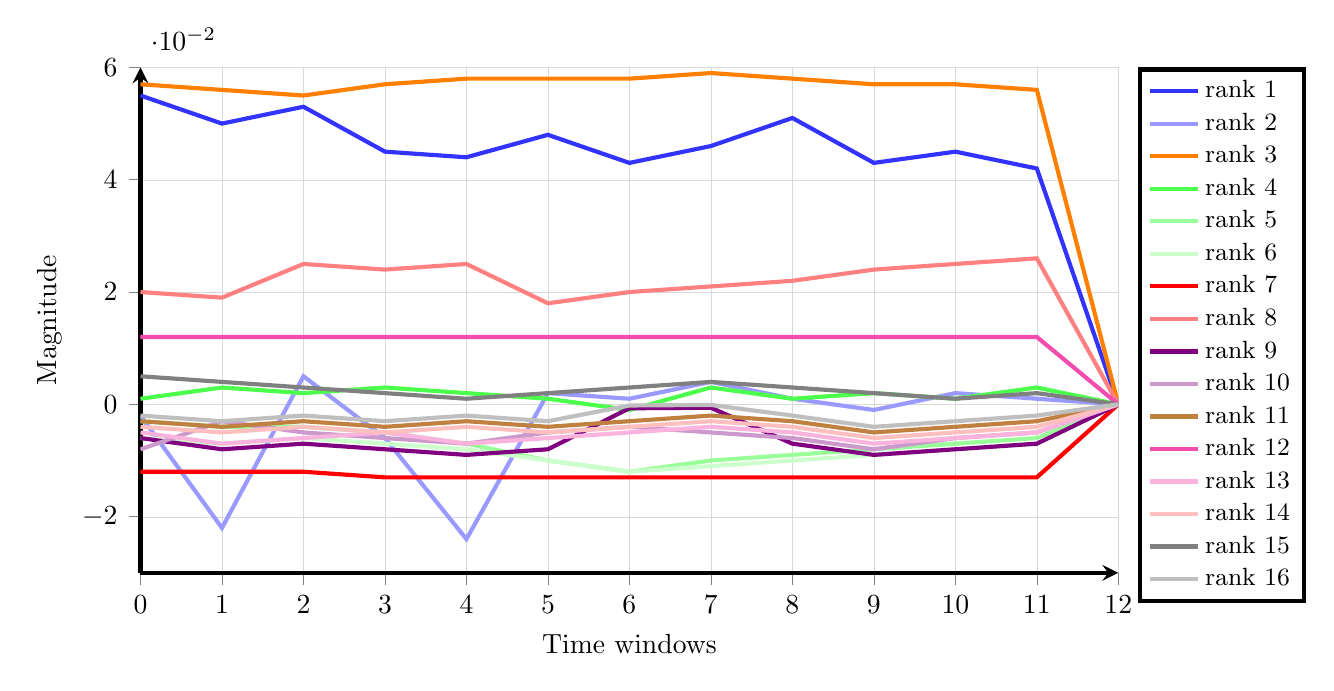
\begin{tikzpicture}
\begin{axis}[
    width=14cm,
    height=8cm,
    xlabel={Time windows},
    ylabel={Magnitude},
    xmin=0, xmax=12,
    ymin=-0.03, ymax=0.06,
    grid=major,
    grid style={line width=0.1pt, draw=gray!30},
    axis lines=left,
    tick align=outside,
    legend style={
        at={(1.02,1)},
        anchor=north west,
        legend columns=1,
        font=\small
    },
    legend cell align=left,
    line width=1.5pt,
]

% Component 1 (bleu foncé)
\addplot[color=blue!80, line width=1.5pt] coordinates {
    (0, 0.055) (1, 0.050) (2, 0.053) (3, 0.045) (4, 0.044) 
    (5, 0.048) (6, 0.043) (7, 0.046) (8, 0.051) (9, 0.043) 
    (10, 0.045) (11, 0.042) (12, 0.000)
};

% Component 2 (bleu clair)
\addplot[color=blue!40, line width=1.5pt] coordinates {
    (0, -0.002) (1, -0.022) (2, 0.005) (3, -0.006) (4, -0.024) 
    (5, 0.002) (6, 0.001) (7, 0.004) (8, 0.001) (9, -0.001) 
    (10, 0.002) (11, 0.001) (12, 0.000)
};

% Component 3 (orange)
\addplot[color=orange, line width=1.5pt] coordinates {
    (0, 0.057) (1, 0.056) (2, 0.055) (3, 0.057) (4, 0.058) 
    (5, 0.058) (6, 0.058) (7, 0.059) (8, 0.058) (9, 0.057) 
    (10, 0.057) (11, 0.056) (12, 0.000)
};

% Component 4 (vert)
\addplot[color=green!70, line width=1.5pt] coordinates {
    (0, 0.001) (1, 0.003) (2, 0.002) (3, 0.003) (4, 0.002) 
    (5, 0.001) (6, -0.001) (7, 0.003) (8, 0.001) (9, 0.002) 
    (10, 0.001) (11, 0.003) (12, 0.000)
};

% Component 4 (vert clair)
\addplot[color=green!40, line width=1.5pt] coordinates {
    (0, -0.003) (1, -0.004) (2, -0.004) (3, -0.005) (4, -0.007) 
    (5, -0.010) (6, -0.012) (7, -0.010) (8, -0.009) (9, -0.008) 
    (10, -0.007) (11, -0.006) (12, 0.000)
};

% Component 5 (vert très clair)
\addplot[color=green!20, line width=1.5pt] coordinates {
    (0, -0.006) (1, -0.007) (2, -0.006) (3, -0.007) (4, -0.008) 
    (5, -0.010) (6, -0.012) (7, -0.011) (8, -0.010) (9, -0.009) 
    (10, -0.008) (11, -0.007) (12, 0.000)
};

% Component 6 (rouge)
\addplot[color=red, line width=1.5pt] coordinates {
    (0, -0.012) (1, -0.012) (2, -0.012) (3, -0.013) (4, -0.013) 
    (5, -0.013) (6, -0.013) (7, -0.013) (8, -0.013) (9, -0.013) 
    (10, -0.013) (11, -0.013) (12, 0.000)
};

% Component 7 (rouge clair)
\addplot[color=red!50, line width=1.5pt] coordinates {
    (0, 0.020) (1, 0.019) (2, 0.025) (3, 0.024) (4, 0.025) 
    (5, 0.018) (6, 0.020) (7, 0.021) (8, 0.022) (9, 0.024) 
    (10, 0.025) (11, 0.026) (12, 0.000)
};

% Component 8 (violet)
\addplot[color=violet, line width=1.5pt] coordinates {
    (0, -0.006) (1, -0.008) (2, -0.007) (3, -0.008) (4, -0.009) 
    (5, -0.008) (6, -0.0007) (7, -0.0006) (8, -0.007) (9, -0.009) 
    (10, -0.008) (11, -0.007) (12, 0.000)
};

% Component 9 (violet clair)
\addplot[color=violet!40, line width=1.5pt] coordinates {
    (0, -0.008) (1, -0.003) (2, -0.005) (3, -0.006) (4, -0.007) 
    (5, -0.005) (6, -0.004) (7, -0.005) (8, -0.006) (9, -0.008) 
    (10, -0.006) (11, -0.005) (12, 0.000)
};

% Component 10 (marron)
\addplot[color=brown, line width=1.5pt] coordinates {
    (0, -0.003) (1, -0.004) (2, -0.003) (3, -0.004) (4, -0.003) 
    (5, -0.004) (6, -0.003) (7, -0.002) (8, -0.003) (9, -0.005) 
    (10, -0.004) (11, -0.003) (12, 0.000)
};

% Component 12 (rose foncé)
\addplot[color=magenta!70, line width=1.5pt] coordinates {
    (0, 0.012) (1, 0.012) (2, 0.012) (3, 0.012) (4, 0.012) 
    (5, 0.012) (6, 0.012) (7, 0.012) (8, 0.012) (9, 0.012) 
    (10, 0.012) (11, 0.012) (12, 0.000)
};

% Component 13 (rose clair)
\addplot[color=magenta!30, line width=1.5pt] coordinates {
    (0, -0.005) (1, -0.007) (2, -0.006) (3, -0.005) (4, -0.007) 
    (5, -0.006) (6, -0.005) (7, -0.004) (8, -0.005) (9, -0.007) 
    (10, -0.006) (11, -0.005) (12, 0.000)
};

% Component 14 (rose très clair)
\addplot[color=pink, line width=1.5pt] coordinates {
    (0, -0.004) (1, -0.005) (2, -0.004) (3, -0.005) (4, -0.004) 
    (5, -0.005) (6, -0.004) (7, -0.003) (8, -0.004) (9, -0.006) 
    (10, -0.005) (11, -0.004) (12, 0.000)
};

% Component 15 (gris)
\addplot[color=gray, line width=1.5pt] coordinates {
    (0, 0.005) (1, 0.004) (2, 0.003) (3, 0.002) (4, 0.001) 
    (5, 0.002) (6, 0.003) (7, 0.004) (8, 0.003) (9, 0.002) 
    (10, 0.001) (11, 0.002) (12, 0.000)
};

% Component 16 (gris clair)
\addplot[color=gray!50, line width=1.5pt] coordinates {
    (0, -0.002) (1, -0.003) (2, -0.002) (3, -0.003) (4, -0.002) 
    (5, -0.003) (6, -0.0002) (7, -0.0001) (8, -0.002) (9, -0.004) 
    (10, -0.003) (11, -0.002) (12, 0.000)
};

\legend{rank 1, rank 2, rank 3,rank 4, rank 5, rank 6, rank 7, rank 8, rank 9, rank 10, rank 11, rank 12, rank 13, rank 14, rank 15, rank 16}
\end{axis}
\end{tikzpicture}
\caption{Temporal Behaviour of CIC-IoT 2024 Normal Traffic: Each colour in the figure represents a temporal mode obtained from the decomposition of the normal traffic tensor for a specific rank ranging from $1$ to $16$, illustrating the evolution of temporal patterns across successive time windows.}
\label{fig:Temporal_features}
\end{figure}



Regarding the source IP mode, as shown in Figure~\ref{fig:source_IP}, the decomposition revealed a highly sparse pattern. Among the 822 source IP addresses, the vast majority exhibited near-zero loadings, indicating minimal contribution to the latent structure. In contrast, a clear concentration of higher loadings was observed between indices 180 and 360, forming distinct spikes. This indicates that only a limited subset of source IPs showed significant activity or relevance in the factor matrix, while the rest remained largely inactive within the analysed time-frame. This suggests that normal network traffic was primarily driven by a limited set of key source hosts and the magnitude ranging from $-800$ to $1200$ across all ranks, indicates that a reasonable number of source devices were active during the one-hour observation window.


\begin{figure}[H]
    \centering    \includegraphics[width=1.2\linewidth]{Source IP mode.png}
    \caption{Source IP Address Behaviour in CIC IoT 2024 Normal Traffic Tensor.
This figure illustrates the source IP factor components extracted from tensor decomposition at different ranks, demonstrating how source IP addresses contribute to normal traffic patterns. Each colour represents a distinct component corresponding to a different rank value.}
    \label{fig:source_IP}
\end{figure}

In the destination IP mode, the decomposition also revealed a highly sparse structure across the 1,313 destination addresses. Although most values remain close to zero, a limited number of components, particularly in ranks 4, 7 and 13, exhibit isolated high-magnitude spikes around indices 1500, 1800, and 2000. These sharp peaks suggest that only a small subset of destination addresses contributes meaningfully to the structure of the normal traffic tensor, reflecting selective interactions captured by specific ranks.

The behavioural patterns identified in both the source and destination modes align with the hub-and-spoke communication model that is commonly observed in IoT environments. This model is characteristic of enterprise IoT deployments, where the majority of devices primarily communicate with centralised servers, gateways, or cloud infrastructures, rather than engaging in distributed peer-to-peer interactions.


\begin{figure}[H]
    \centering
    \includegraphics[width=1.2\linewidth]{Destination IP mode.png}
   \caption{Destination IP Address Behaviour in the CIC IoT 2024 Normal Traffic Tensor: This figure shows the destination IP address factors for each rank of the tensor decomposition. Each colour represents a specific rank and illustrates how the destination IP addresses contribute to the normal traffic behaviour.}
\end{figure}

Focusing on the features mode, the decomposition revealed diverse behaviours across the four selected features. As shown in Figure~\ref{fig:ranks_evolution}, components from different decomposition ranks (1 to 16) emphasise various combinations of features. Most components either vanish at feature index~1 and peak at feature index~2, or exhibit the inverse pattern. Notably, the components corresponding to ranks~2 and~4 (depicted by the light blue and orange curves) consistently dominate in magnitude, peaking at feature~1 and vanishing at feature~2. These variations indicate that network traffic comprises multiple distinct communication profiles. In particular, some components highlight specific feature combinations, corresponding to different categories of legitimate network activity, such as bulk data transfers (characterised by high bytes per second and longer durations), interactive sessions (marked by high packets per second and shorter durations), or periodic maintenance traffic. This multi-modal characterisation provides a comprehensive representation of legitimate behaviours, thereby facilitating the detection of anomalous feature combinations that deviate from all established normal patterns.

\begin{figure}[H]
\centering
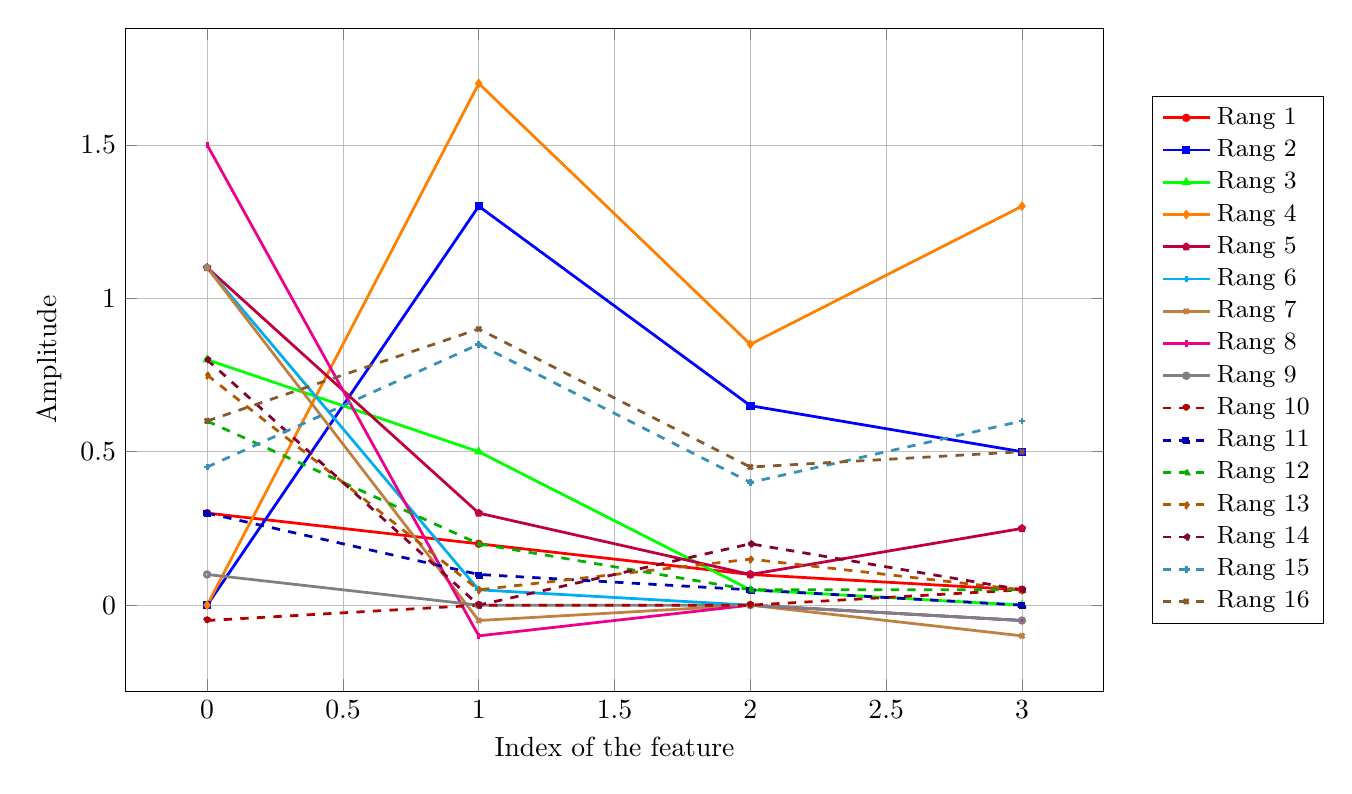
\begin{tikzpicture}
\begin{axis}[
    xlabel={Index of the feature},
    ylabel={Amplitude},
    width=14cm,
    height=10cm,
    grid=both,
    grid style={line width=.1pt, draw=gray!30},
    major grid style={line width=.2pt,draw=gray!50},
    legend style={
        at={(1.05,0.5)},
        anchor=west,
        legend columns=1,
        font=\small
    },
    legend cell align={left},
]

% --- Courbes avec traits plus fins et marqueurs adaptés ---
% Rank 1
\addplot[red, mark=*, mark size=1pt, line width=1pt] coordinates {(0,0.3)(1,0.2)(2,0.1)(3,0.05)};
\addlegendentry{Rang 1}

% Rank 2
\addplot[blue, mark=square*, mark size=1pt, line width=1pt] coordinates {(0,0)(1,1.3)(2,0.65)(3,0.5)};
\addlegendentry{Rang 2}

% Rank 3
\addplot[green, mark=triangle*, mark size=1pt, line width=1pt] coordinates {(0,0.8)(1,0.5)(2,0.05)(3,0.0)};
\addlegendentry{Rang 3}

% Rank 4
\addplot[orange, mark=diamond*, mark size=1pt, line width=1pt] coordinates {(0,0)(1,1.7)(2,0.85)(3,1.3)};
\addlegendentry{Rang 4}

% Rank 5
\addplot[purple, mark=pentagon*, mark size=1pt, line width=1pt] coordinates {(0,1.1)(1,0.3)(2,0.1)(3,0.25)};
\addlegendentry{Rang 5}

% Rank 6
\addplot[cyan, mark=+, mark size=1.2pt, line width=1pt] coordinates {(0,1.1)(1,0.05)(2,0.0)(3,-0.05)};
\addlegendentry{Rang 6}

% Rank 7
\addplot[brown, mark=x, mark size=1.2pt, line width=1pt] coordinates {(0,1.1)(1,-0.05)(2,0.0)(3,-0.1)};
\addlegendentry{Rang 7}

% Rank 8
\addplot[magenta, mark=|, mark size=1.2pt, line width=1pt] coordinates {(0,1.5)(1,-0.1)(2,0.0)(3,-0.05)};
\addlegendentry{Rang 8}

% Rank 9
\addplot[gray, mark=o, mark size=1pt, line width=1pt] coordinates {(0,0.1)(1,0.0)(2,0.0)(3,-0.05)};
\addlegendentry{Rang 9}

% Rangs 10-16 avec traits fins et style dashed
\addplot[red!70!black, mark=*, mark size=1pt, line width=1pt, dashed] coordinates {(0,-0.05)(1,0.0)(2,0.0)(3,0.05)};
\addlegendentry{Rang 10}

\addplot[blue!70!black, mark=square*, mark size=1pt, line width=1pt, dashed] coordinates {(0,0.3)(1,0.1)(2,0.05)(3,0.0)};
\addlegendentry{Rang 11}

\addplot[green!70!black, mark=triangle*, mark size=1pt, line width=1pt, dashed] coordinates {(0,0.6)(1,0.2)(2,0.05)(3,0.05)};
\addlegendentry{Rang 12}

\addplot[orange!70!black, mark=diamond*, mark size=1pt, line width=1pt, dashed] coordinates {(0,0.75)(1,0.05)(2,0.15)(3,0.05)};
\addlegendentry{Rang 13}

\addplot[purple!70!black, mark=pentagon*, mark size=1pt, line width=1pt, dashed] coordinates {(0,0.8)(1,0.0)(2,0.2)(3,0.05)};
\addlegendentry{Rang 14}

\addplot[cyan!70!black, mark=+, mark size=1.2pt, line width=1pt, dashed] coordinates {(0,0.45)(1,0.85)(2,0.4)(3,0.6)};
\addlegendentry{Rang 15}

\addplot[brown!70!black, mark=x, mark size=1.2pt, line width=1pt, dashed] coordinates {(0,0.6)(1,0.9)(2,0.45)(3,0.5)};
\addlegendentry{Rang 16}

\end{axis}
\end{tikzpicture}
\caption{Features Behaviour in CIC IoT 2024 Traffic: This figure shows how the magnitude of features varies across latent factors for each rank considered in the tensor decomposition. Each component is represented by a different colour.}
\label{fig:ranks_evolution}
\end{figure}


\noindent After decomposing the normal tensor and identifying the corresponding normal latent space, we proceeded to the projection step by projecting both the train and test tensors onto this space for ranks ranging from $1$ to $16$. Figures~\ref{fig:train-error} and ~\ref{fig:test-error} illustrate the evolution of the projection norm as a function of the rank. There show a non-monotonic and erratic evolution of the projection norm across ranks, with values ranging from 50 to 150 and peaking at rank 13. This behaviour was expected for two main reasons. First, the projection process is sensitive to the scale of the factor matrices $\mathbf{B}$, $\mathbf{C}$, and $\mathbf{D}$. The use of the Khatri-Rao product and the Moore-Penrose pseudoinverse amplifies this sensitivity, especially when the matrices are poorly conditioned or contain unstable values. Second, both the training and testing tensors contain more attack data than normal traffic. Since the latent space was constructed to represent normal behaviour, many vectors are poorly projected, resulting in higher reconstruction errors. Hence, since the reconstruction error during the decomposition process ranged from $0.3$ to $0.1$, all our decompositions can be considered acceptable. This suggests that some of the corresponding projections are more likely to be relevant and better aligned with the normal latent space than others.


\begin{figure}[H]
    \centering
    \begin{subfigure}[t]{0.48\linewidth}
        \centering
        \includegraphics[width=\linewidth]{projection test plot.png}
        \caption{Training projection norm across different tensor ranks.}
        \label{fig:train-error}
    \end{subfigure}
    \hfill
    \begin{subfigure}[t]{0.48\linewidth}
        \centering
        \includegraphics[width=\linewidth]{projection test plot.png}
        \caption{Test projection norm across different tensor ranks.}
        \label{fig:test-error}
    \end{subfigure}
    \caption{Projection Norms Across Different Tensor Ranks for the Train and Test Tensors: This figure illustrates the projection norms into the normal latent space for both the training and testing tensors across different ranks, highlighting how the choice of rank affects the representation of the latent space.}
    \label{fig:projection-norms}
\end{figure}
\noindent Once projection step completed, we computed the corresponding residuals. Figures~\ref{fig:train-residuals} and ~\ref{fig:test-residuals} illustrate the evolution of the residual norms across varying ranks. Since the projection curves were not smooth across ranks, the residual curves exhibited similarly irregular behaviour.
\begin{figure}[H]
    \centering
    \begin{subfigure}[t]{0.48\linewidth}
        \centering
        \includegraphics[width=\linewidth]{train errors.png}
        \caption{ Training Projection Error across different tensor ranks.}
        \label{fig:train-residuals}
    \end{subfigure}
    \hfill
    \begin{subfigure}[t]{0.48\linewidth}
        \centering
        \includegraphics[width=\linewidth]{test error.png}
        \caption{Testing Projection Error across different tensor ranks.}
        \label{fig:test-residuals}
    \end{subfigure}
    \caption{Projection Error for Train and Test Tensors Across Different Tensor Ranks (Scale $10^{-1}$): This figure illustrates the projection error for both the training and testing tensors across different ranks, showing how the choice of rank affects the reconstruction error in the latent space.}
    \label{fig:train-test-residual}
\end{figure}
 
\subsection{Anomaly Detection And Rank selection Results}
 Following the aggregation step, sixteen deep learning models were trained, each corresponding to a specific rank of tensors. Their performance was assessed using standard metrics: accuracy, precision, recall, and F1-score. Figure~\ref{fig:confusion_matrices_1}, ~\ref{fig:confusion_matrices_2} and ~\ref{fig:confusion_matrices_3} present the confusion matrices for all sixteen models. These matrices reveal low false positives and a number of false negatives ranging from 5 to 13, indicating that all models achieved good performance in distinguishing between attack and non-attack traffic.

% Figure 1 : Ranks 1–2
% Figure 1 : Ranks 1–6
\begin{figure}[H]
    \centering
    \begin{tabular}{ccc}
        \includegraphics[width=0.3\linewidth]{rank_1.png} &
        \includegraphics[width=0.3\linewidth]{rank_2.png} &
        \includegraphics[width=0.3\linewidth]{rank_3.png} \\
        \small Rank 1 & \small Rank 2 & \small Rank 3 \\[6pt]
    \end{tabular}
    \caption{Confusion Matrices for Tensor Ranks 1–3: This figure presents the confusion matrices for tensor ranks 1 to 3, illustrating the classification performance of the models for each rank.}
    \label{fig:confusion_matrices_1}
\end{figure}

% Figure 2 : Ranks 7–12
\begin{figure}[H]
    \centering
    \begin{tabular}{ccc}
        \includegraphics[width=0.3\linewidth]{rank_4.png} &
        \includegraphics[width=0.3\linewidth]{rank_5.png} &
        \includegraphics[width=0.3\linewidth]{rank_6.png} \\
        \small Rank 4 & \small Rank 5 & \small Rank 6 \\[3pt]

        \includegraphics[width=0.3\linewidth]{rank_7.png} &
        \includegraphics[width=0.3\linewidth]{rank_8.png} &
        \includegraphics[width=0.3\linewidth]{rank_9.png} \\
        \small Rank 7 & \small Rank 8 & \small Rank 9 \\[3pt]

        \includegraphics[width=0.3\linewidth]{rank_10.png} &
        \includegraphics[width=0.3\linewidth]{rank_11.png} &
        \includegraphics[width=0.3\linewidth]{rank_12.png} \\
        \small Rank 10 & \small Rank 11 & \small Rank 12
    \end{tabular}
    \caption{Confusion matrices for tensor ranks 4–12, showing the classification performance of the models for each rank.}
    \label{fig:confusion_matrices_2}
\end{figure}


% Figure 3 : Ranks 13–16
\begin{figure}[H]
    \centering
    \begin{tabular}{ccc}
        \includegraphics[width=0.3\linewidth]{rank_13.png} &
        \includegraphics[width=0.3\linewidth]{rank_14.png} &
        \includegraphics[width=0.3\linewidth]{rank_15.png} \\
        \small Rank 13 & \small Rank 14 & \small Rank 15 \\[6pt]

        \includegraphics[width=0.3\linewidth]{rank_16.png} & & \\
        \small Rank 16 & & 
    \end{tabular}
    \caption{Confusion Matrices for Tensor Ranks 13–16: This figure presents the confusion matrices for tensor ranks 13 to 16, illustrating the classification performance of the models for each rank.}
    \label{fig:confusion_matrices_3}
\end{figure}


 Figure~\ref{fig:accl} presents the accuracy of each of the models. As shown, all models achieve accuracy values ranging from 99.90\% to 99.96\% respectively achieved by model 1 and model 9, which confirms the performance trends observed in the confusion matrices.
\begin{figure}[H]
    \centering
    \includegraphics[width=1.1\linewidth]{accu.png}
    \caption{Accuracy of each model: This figure illustrates the accuracy scores obtained by each trained model. It provides an overall view of how well each model classifies both normal and anomalous traffic, highlighting the rank that yields the highest predictive performance.}
    \label{fig:accl}
\end{figure}
\noindent Additionally, Figures~\ref{fig:recall} and ~\ref{fig:f1} present the recall, and F1-score for each model, respectively. All models achieve good recall with values ranging from 99.03\% to 99.63\%, demonstrating the models’ strong capability to detect nearly all attacks, with Model 9 achieving the highest recall. Similarly, the F1-scores range from 99.51\% to 99.81\%, with Model 9 again achieving the best performance, confirming its overall superiority.

% Figure 2 : Recall
\begin{figure}[H]
    \centering
    \includegraphics[width=1.1\linewidth]{recall.png}
    \caption{Recall of each model: This figure presents the recall achieved by each trained model. It highlights the models’ ability to correctly identify anomalous traffic, emphasising which rank provides the most reliable detection performance.}
    \label{fig:recall}
\end{figure}

% Figure 3 : F1-score
\begin{figure}[H]
    \centering
    \includegraphics[width=1\linewidth]{F1-score.png}
    \caption{F1-scores of each model: This figure illustrates the F1-score obtained for each trained model. It highlights the variation in performance and identifies the rank that yields the best balance between precision and recall.}
    \label{fig:f1}
\end{figure}
To facilitate a comprehensive comparison of the models, the summary results are presented in Table~\ref{tab:model_comparison}. This consolidated table of performance metrics provides a clear overview of each model’s evaluation scores and highlights the trade-off between the true positive rate (sensitivity) and the false positive rate, thereby offering insight into each model’s ability to distinguish between attack and normal traffic.

\begin{table}
\caption{Models performance summary table: This table summarises the performance of each trained model. It reports the accuracy, recall, and F1-score of each model, and highlights Model 9 as the best-performing one.}\label{tab:model_comparison}
\begin{tabular}{@{}lllll@{}}
\toprule
\textbf{Rank} & \textbf{Model} & \textbf{Accuracy[\%]} & \textbf{Recall[\%]} & \textbf{F1 Score[\%]} \\
\midrule
1 & Model\_1 & 0.9990 & 0.9903 & 0.9951 \\
2 & Model\_2 & 0.9992 & 0.9925 & 0.9962 \\
3 & Model\_3 & 0.9994 & 0.9940 & 0.9970 \\
4 & Model\_4 & 0.9993 & 0.9933 & 0.9966 \\
5 & Model\_5 & 0.9994  & 0.9940 & 0.9970 \\
6 & Model\_6 & 0.9992  & 0.9925 & 0.9962 \\
7 & Model\_7 & 0.9993 & 0.9933 & 0.9966 \\
8 & Model\_8 & 0.9992 & 0.9925 & 0.9962 \\
9 & Model\_9 & 0.9996  & 0.9963 & 0.9981 \\
10 & Model\_10 & 0.9994 & 0.9940 & 0.9970 \\
11 & Model\_11 & 0.9994 & 0.9940 & 0.9970 \\
12 & Model\_12 & 0.9994 & 0.9940 & 0.9970 \\
13 & Model\_13 & 0.9993 & 0.9933 & 0.9966 \\
14 & Model\_14 & 0.9993 & 0.9933 & 0.9966 \\
15 & Model\_15 & 0.9995 & 0.9948 & 0.9974 \\
16 & Model\_16 & 0.9994 & 0.9940 & 0.9970 \\
\bottomrule
\end{tabular}
\end{table}

In summary, all the models demonstrated high performance across all metrics, with accuracy, recall, and F1-score values ranging from 99.90\% to 100\%. However, some models performed slightly less well than others. For instance, Model 1 exhibited relatively lower performance compared to the rest, and this trend continued across the subsequent models until Model 9, which achieved the highest scores across all metrics, marking it as the most effective model in the set.  

The best performance was achieved at rank 9, with 99.96\% accuracy and 99.63\% recall, indicating that this rank offers an optimal balance between capturing sufficient complexity in the normal behaviour model and avoiding overfitting. Consequently, the projection at rank 9 was identified as the best performing model for anomaly detection, which aligns well with the findings of \cite{eren2023general}, who similarly evaluated multiple ranks ranging from 1 to 100 in steps of 5 and determined an expected optimal rank around 50. 

 The gradual improvement in recall from Rank 1 (99.03\%) to Rank 9 (99.63\%) followed by stabilization suggests that higher-rank decompositions capture increasingly subtle patterns in normal behaviour, enhancing the model's ability to distinguish between legitimate and anomalous activities. However, the diminishing returns beyond Rank 9 indicates that additional complexity does not necessarily translate to improved performance, supporting the selection of Rank 9 as the optimal configuration.   

\subsection{Comparison with the state-of-the-art}

We compared our proposed framework with state-of-the-art methods. For this comparison, four baseline models were selected: Decision Tree, Random Forest, Support Vector Machine (SVM), and Long Short-Term Memory (LSTM). The corresponding confusion matrices for these models are presented in Figure~\ref{fig:confusion_matrices_tree_forest}, ~\ref{fig:confusion_matrices_svm_lstm}.

% Première figure avec Decision Tree et Random Forest
\begin{figure}[H]
    \centering
    \begin{tabular}{cc}
        \includegraphics[width=0.5\linewidth]{Decision tree.png} &
        \includegraphics[width=0.5\linewidth]{Random Forest.png} \\
        \small Decision Tree & \small Random Forest
    \end{tabular}
    \caption{Confusion matrices of Decision Tree and Random Forest:
This figure shows the performance of both models in classifying normal and anomalous traffic.}
    \label{fig:confusion_matrices_tree_forest}
\end{figure}

% Deuxième figure avec SVM et LSTM
\begin{figure}[H]
    \centering
    \begin{tabular}{cc}
        \includegraphics[width=0.5\linewidth]{support vector Machine.png} &
        \includegraphics[width=0.5\linewidth]{LSTM.png} \\
        \small Support Vector Machine & \small LSTM
    \end{tabular}
    \caption{Confusion Matrices of Support Vector Machine and LSTM:
This figure illustrates the performance of both models in classifying normal and anomalous traffic.}
    \label{fig:confusion_matrices_svm_lstm}
\end{figure}


\noindent The comparison between our model and the baseline models was conducted using false positive and false negative rates. Figure~\ref{fig:fp_fn_comparison} illustrates the distribution of these rates across the different models.
\begin{figure}[H]
    \centering
    \includegraphics[width=1.05\linewidth]{compa3.png}
    \caption{False Positive and False Negative Rates Across Classification Models:
This figure summarizes the comparison between our model and state-of-the-art approaches in terms of false positives and false negatives. False positives are represented by the red bands, while false negatives are shown in blue. The results highlight how our method outperforms traditional approaches.}
    \label{fig:fp_fn_comparison}
\end{figure}
\noindent The comparison with baseline models shows that our method achieves a notable reduction in false positives. While the Decision Tree, Random Forest, SVM, and LSTM models recorded false positive rates of 78.3\%, 70.1\%, 100\%, and 44.6\% respectively, our approach achieved a rate of 0\%. 

In terms of false negatives, our method reported a rate of 0.37\%, which is slightly higher than those observed in the other models: 0.11\% for Decision Tree, 0.10\% for Random Forest, 0\% for SVM, and 0.12\% for LSTM. Consequently, the recall of our method is slightly lower than that of the baselines, but remains within a reasonable range.


Overall, the results indicate that our approach effectively minimises false alarms while maintaining strong detection capability. This comparison  reveals important insights about the practical effectiveness of our model versus traditional methods. 

Achieving a low false positive rate indicates that our approach helps reduce false alarms, which are a common challenge in anomaly detection and can lead to wasted resources and diminished trust in security systems. The low false negative rate of 0.37\% further indicates that our model reliably detects nearly all true anomalies, striking an excellent balance between sensitivity and precision.

In contrast, the baseline methods exhibit notable limitations. SVM suffers from a very high false positive rate, limiting its practical applicability. Decision Tree and Random Forest are affected by overfitting, leading to frequent false alarms and missed detections. Even LSTM, despite its more complex architecture, yields a false positive rate that remains relatively high for reliable operational use.

 The strong performance of our model can be primarily attributed to the tensor-based approach, which naturally preserves the multi-dimensional structure of network traffic data as discussed earlier. The projection step allowed us to clearly capture the network signature, effectively distinguishing normal from anomalous behaviours. Moreover, the IP aggregation technique provided a comprehensive view of communication patterns, enhancing the model’s sensitivity to subtle deviations. 
 
 These methodological strengths grounded in the tensor decomposition and aggregation framework presented in previous sections, explain the expected and impressive results achieved by our method. The modest increase in false negatives to 0.37\% represents a strategically sound trade-off that maintains good sensitivity (99.63\% recall) while achieving perfect precision. This trade-off profile is particularly valuable in security applications where the cost of false alarms often exceeds the cost of occasionally missing an attack, especially when the miss rate remains below 0.4\%.


The flexibility and high performance of our method directly address key practical requirements for real-world deployment. First, the complete elimination of false positives significantly enhances operational efficiency by removing the need for manual investigation of false alarms, thereby supporting the implementation of automated response mechanisms. This perfect precision also reinforces system credibility, maintaining operator trust and avoiding the alert fatigue that often results from high false alarm rates. Moreover, by eliminating the burden of false positive management, the method facilitates scalability, allowing the system to be deployed across larger infrastructures without requiring a proportional increase in human oversight. Finally, the combined effect of reduced investigation costs and improved operational efficiency yields substantial economic benefits, making our approach highly cost-effective compared to traditional baselines.


The results obtained from our tensor-based anomaly detection framework reveal important patterns and relationships within the dynamic network traffic under investigation. Notably, we observe that anomalies such as DDoS and DoS attacks exhibit both spatial and temporal regularities. Temporally, attacks often appear in burst patterns, marked by sudden increases in flow count or packet rates. Spatially, anomalies consistently cluster around specific Destination IPs, which act as focal points of malicious activity. These observations suggest that traffic anomalies are not uniformly distributed but are instead localized in time and space.

One of the major findings of our study is the effectiveness of performing aggregation after calculating the residue tensor, particularly across the Source IP dimension. This approach consistently improved anomaly score stability and detection accuracy. Unlike the method proposed in~\cite{streit2021network}, which omits post-projection aggregation, our strategy leverages this step to consolidate residuals along critical dimensions. This post-processing facilitates the isolation of malicious behaviour signatures more effectively, as residual anomalies often cluster around specific destinations.Furthermore, our framework incorporates a deep learning-driven rank selection mechanism, which dynamically adapts the model complexity to the intrinsic structure of the network traffic data. This approach allows us to effectively select the rank that aligns perfectly with the deep learning model.


Despite the encouraging results of our approach, several limitations must be acknowledged. First, our method is based on the extraction of normal traffic to construct a latent reference space. However, normal network traffic is inherently dynamic and subject to variations due to changes in user behaviour, application usage, and service demands. This non-stationary nature of benign traffic complicates the definition of a stable normal model, which may lead to misclassification, as previously highlighted in works such as~\cite{limitation2023generalization}. Additionally, our study focuses solely on DDoS and DDoS HTTP Flood attack types. While our method demonstrates strong performance for these categories, it may not generalize well to other types of attacks, particularly stealthy or low-rate DoS attacks, which tend to exhibit subtle deviations from normal behaviour~\cite{al2021machine}. These forms of attacks often bypass detection due to their weak anomaly signatures. Furthermore, unlike~\cite{streit2021network}, we perform aggregation across the Destination IP dimension after projection to improve anomaly signature preservation. Although this design choice enhances stability and efficiency, it may not capture complex temporal relationships present in the raw data. These limitations highlight the need for complementary research on adaptive normal space extraction, as well as the evaluation and adaptation of the model to other types of attacks.

The patterns observed in our anomaly detection results can be attributed to several key mechanisms. First the diversity of ranks used in the CP factorization allowed us to explore a range of latent space configurations, increasing the chances of accurately modelling normal network behaviour. Second, aggregation along the Destination IP dimension, performed after projection on the residuals, significantly allows us to obtain simple datasets which served as input of our deep learning models. Finally, our deep learning architecture was carefully designed, incorporating dense layers, appropriate non-linear activation functions, batch normalization, dropout, and well-optimized classification heads, enabling effective use of the extracted features. The combination of these mechanisms played a crucial role in the robustness and precision of the model predictions.

Our approach is consistent with a growing body of research advocating tensor methods in cybersecurity, but it also introduces important modifications. In particular, our combination of the 4D projection,aggregation and rank  selection guided by  our work from existing literature. Moreover, this methodological refinement suggests a general principle: that intelligently structuring data prior to decomposition can improve model performance without sacrificing interpretability.

The proposed methodology integrates efficient preprocessing, dimensionality reduction, and latent space modelling to detect anomalies with both high performance and flexibility. These contributions have implications that extend beyond cybersecurity. Domains such as environmental monitoring, fraud detection, and intelligent transportation systems, which also involve high-dimensional and time-varying data, may benefit from the adoption of similar modelling strategies.



Nevertheless, we remain cautious in interpreting our findings. While the results strongly support the proposed pipeline, alternative explanations are possible. For example, the observed improvement may stem from specific characteristics of the CIC IoT 2024 dataset. To mitigate this limitation, future work should explore the generalizability of our approach across different datasets and attack scenarios.

\section{Conclusion}
This research has brought significant advances in tensor decomposition-based anomaly detection applied to network traffic analysis. Our methodological framework demonstrated robust capabilities in  detection anomalies in network traffic with acceptable false positive rates. We specifically worked on a network comprising 105 IoT devices, representing a complex and realistic environment. However, scaling this approach to real-world Internet networks with a much larger number of devices would require increased computational and hardware resources to handle the data volume and velocity. 

We should also noted other limitations, the evaluation of our model was mainly conducted on the CIC IoT-IDAD 2024 dataset, which may limit the generalizability of the results to other network architectures and contexts. Moreover, our approach relies on the extraction of normal traffic, which can be challenging due to the highly dynamic nature of real-world network traffic. Additionally, the attack types studied (DoS and DDoS HTTP Flood) do not cover the full range of modern cyber threats, and real operational conditions introduce further challenges such as network congestion and legitimate traffic anomalies.

To deepen and enhance this approach, several research directions are envisaged: developing adaptive models for normal traffic extraction capable of tracking its dynamic changes; integrating robust methods to manage high data volume and speed; designing adaptive tensor-based classification techniques able to automatically identify various attack types and malicious devices; validating the method on larger, more heterogeneous real networks; and extending applications to other domains dealing with complex multi-dimensional data. These perspectives pave the way for more flexible, accurate, and scalable anomaly detection systems suited to the increasing demands of current and future network environments.

Based on the findings and limitations of this research, future work should focus on: Dataset Diversification and Validation, evaluate the approach on diverse datasets and real-world networks, surpassing the 105 IoT devices studied here, to validate generalizability and address increased hardware and computational resource demands.

\noindent Extend detection to advanced persistent threats, multi-stage, polymorphic, and insider attacks, requiring more advanced temporal models and adaptive mechanisms.
   
\noindent Develop models capable of adaptively extracting normal behaviours despite the dynamic and variable nature of real-world traffic, which remains a major challenge.
    

\noindent Explore tensor-based methods that not only classify various attack types effectively but also precisely identify malicious devices within the network. This would enhance fine-grained detection and targeted response to threats.
    
\noindent Design frameworks for real-time deployment, hybrid architectures integrating existing security tools, and adaptations for resource-constrained edge computing environments.
    
\noindent Incorporate online learning, uncertainty quantification, and explainable AI to improve robustness, interpretability, and continuous adaptation.
    
\noindent Investigate hardware acceleration, distributed processing, and model compression to enable scalable and efficient solutions for large-scale networks.

\backmatter

% \bmhead{Acknowledgements}
% Thanks the National Research Foundation of South Africa for support through project number CSRP23040990793.

\section*{Declarations}

\subsection*{Data availability}
The data used in our study are publicly available and can be accessed at \url{http://cicresearch.ca/IOTDataset/CIC%20IoT-IDAD%20Dataset%202024/}. This dataset, known as the CIC IoT-IDAD 2024 Dataset, provides a comprehensive collection of IoT network traffic, including both normal and malicious patterns, making it suitable for anomaly detection and cybersecurity research.

% \subsection*{Author contributions}
% \textbf{Jospin Price Yonel Mitsouma:} Conceptualization, Data curation, Formal analysis, Investigation, Methodology, Software, Visualisation, Writing -- original draft, Writing -- review \& editing. \textbf{Pouya Ataei:} Conceptualization, Methodology, Formal analysis, Visualisation, Writing--review \& editing, Supervision, Coding, Creating the Actual Pipeline, Mathematics, Validation. \textbf{Marcellin Atemkeng:} Conceptualization, Methodology, Visualisation, Formal analysis, Writing -- review \& editing, Supervision, Validation. \textbf{Emmanuel Fouotsa:} Resources, Writing -- review \& editing, Validation, Funding acquisition, Supervision.

\bibliography{References}

\end{document}
